\usetikzlibrary{calc}
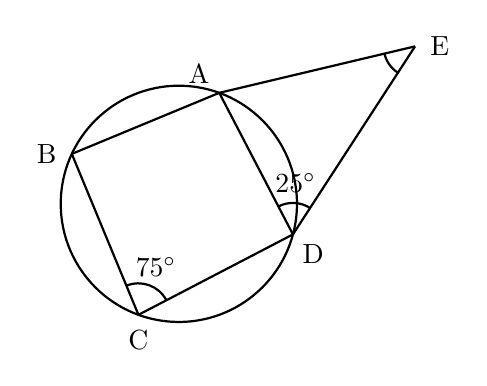
\begin{tikzpicture}[scale=1]

    % Define the center of the circle
    \coordinate (O) at (0,0);

    % Draw the circle
    \draw[thick] (O) circle (1.5);

    % Define points A, B, C, D on the circle
    \coordinate (A) at (70:1.5);
    \coordinate (B) at (155:1.5);
    \coordinate (C) at (250:1.5);
    \coordinate (D) at (345:1.5);

    % External point E
    \coordinate (E) at (3, 2);

    % Draw the cyclic quadrilateral sides and extensions
    \draw[thick] (B) -- (C);
    \draw[thick] (A) -- (D);
    \draw[thick] (B) -- (A);
    \draw[thick] (C) -- (D);
    \draw[thick] (E) -- (A);
    \draw[thick] (E) -- (D);

    % --- Precise angle arcs ---

    % Angle BCD at C
    % C->D direction: atan2(1.0213, 1.9619) = 27.5°
    % C->B direction: atan2(2.0435, -0.8464) = 112.5°
    \draw[thick] ($(C) + (27.5:0.4)$) arc (27.5:112.5:0.4);

    % Angle ADE at D
    % D->E direction: atan2(2.3882, 1.5511) = 57°
    % D->A direction: atan2(1.7978, -0.9359) = 117.5°
    \draw[thick] ($(D) + (57:0.4)$) arc (57:117.5:0.4);

    % Angle AED at E
    % E->A direction: atan2(-0.5905, -2.487) = 193.35°
    % E->D direction: atan2(-2.3882, -1.5511) = 237°
    \draw[thick] ($(E) + (193.35:0.4)$) arc (193.35:237:0.4);

    % Add labels for the points
    \node[above left] at (A) {A};
    \node[left, xshift=-2pt] at (B) {B};
    \node[below, yshift=-2pt] at (C) {C};
    \node[below right] at (D) {D};
    \node[right, xshift=2pt] at (E) {E};

    % Add angle values
    \node at ($(C) + (70:0.65)$) {$75^{\circ}$};
    \node at ($(D) + (87:0.65)$) {$25^{\circ}$};

\end{tikzpicture}